% Options for packages loaded elsewhere
\PassOptionsToPackage{unicode}{hyperref}
\PassOptionsToPackage{hyphens}{url}
\PassOptionsToPackage{dvipsnames,svgnames,x11names}{xcolor}
%
\documentclass[
  letterpaper,
  DIV=11,
  numbers=noendperiod]{scrreprt}

\usepackage{amsmath,amssymb}
\usepackage{lmodern}
\usepackage{iftex}
\ifPDFTeX
  \usepackage[T1]{fontenc}
  \usepackage[utf8]{inputenc}
  \usepackage{textcomp} % provide euro and other symbols
\else % if luatex or xetex
  \usepackage{unicode-math}
  \defaultfontfeatures{Scale=MatchLowercase}
  \defaultfontfeatures[\rmfamily]{Ligatures=TeX,Scale=1}
\fi
% Use upquote if available, for straight quotes in verbatim environments
\IfFileExists{upquote.sty}{\usepackage{upquote}}{}
\IfFileExists{microtype.sty}{% use microtype if available
  \usepackage[]{microtype}
  \UseMicrotypeSet[protrusion]{basicmath} % disable protrusion for tt fonts
}{}
\makeatletter
\@ifundefined{KOMAClassName}{% if non-KOMA class
  \IfFileExists{parskip.sty}{%
    \usepackage{parskip}
  }{% else
    \setlength{\parindent}{0pt}
    \setlength{\parskip}{6pt plus 2pt minus 1pt}}
}{% if KOMA class
  \KOMAoptions{parskip=half}}
\makeatother
\usepackage{xcolor}
\setlength{\emergencystretch}{3em} % prevent overfull lines
\setcounter{secnumdepth}{5}
% Make \paragraph and \subparagraph free-standing
\ifx\paragraph\undefined\else
  \let\oldparagraph\paragraph
  \renewcommand{\paragraph}[1]{\oldparagraph{#1}\mbox{}}
\fi
\ifx\subparagraph\undefined\else
  \let\oldsubparagraph\subparagraph
  \renewcommand{\subparagraph}[1]{\oldsubparagraph{#1}\mbox{}}
\fi


\providecommand{\tightlist}{%
  \setlength{\itemsep}{0pt}\setlength{\parskip}{0pt}}\usepackage{longtable,booktabs,array}
\usepackage{calc} % for calculating minipage widths
% Correct order of tables after \paragraph or \subparagraph
\usepackage{etoolbox}
\makeatletter
\patchcmd\longtable{\par}{\if@noskipsec\mbox{}\fi\par}{}{}
\makeatother
% Allow footnotes in longtable head/foot
\IfFileExists{footnotehyper.sty}{\usepackage{footnotehyper}}{\usepackage{footnote}}
\makesavenoteenv{longtable}
\usepackage{graphicx}
\makeatletter
\def\maxwidth{\ifdim\Gin@nat@width>\linewidth\linewidth\else\Gin@nat@width\fi}
\def\maxheight{\ifdim\Gin@nat@height>\textheight\textheight\else\Gin@nat@height\fi}
\makeatother
% Scale images if necessary, so that they will not overflow the page
% margins by default, and it is still possible to overwrite the defaults
% using explicit options in \includegraphics[width, height, ...]{}
\setkeys{Gin}{width=\maxwidth,height=\maxheight,keepaspectratio}
% Set default figure placement to htbp
\makeatletter
\def\fps@figure{htbp}
\makeatother

\usepackage{float}
\raggedbottom
\KOMAoption{captions}{tableheading}
\makeatletter
\makeatother
\makeatletter
\@ifpackageloaded{bookmark}{}{\usepackage{bookmark}}
\makeatother
\makeatletter
\@ifpackageloaded{caption}{}{\usepackage{caption}}
\AtBeginDocument{%
\ifdefined\contentsname
  \renewcommand*\contentsname{Table of contents}
\else
  \newcommand\contentsname{Table of contents}
\fi
\ifdefined\listfigurename
  \renewcommand*\listfigurename{List of Figures}
\else
  \newcommand\listfigurename{List of Figures}
\fi
\ifdefined\listtablename
  \renewcommand*\listtablename{List of Tables}
\else
  \newcommand\listtablename{List of Tables}
\fi
\ifdefined\figurename
  \renewcommand*\figurename{Figure}
\else
  \newcommand\figurename{Figure}
\fi
\ifdefined\tablename
  \renewcommand*\tablename{Table}
\else
  \newcommand\tablename{Table}
\fi
}
\@ifpackageloaded{float}{}{\usepackage{float}}
\floatstyle{ruled}
\@ifundefined{c@chapter}{\newfloat{codelisting}{h}{lop}}{\newfloat{codelisting}{h}{lop}[chapter]}
\floatname{codelisting}{Listing}
\newcommand*\listoflistings{\listof{codelisting}{List of Listings}}
\makeatother
\makeatletter
\@ifpackageloaded{caption}{}{\usepackage{caption}}
\@ifpackageloaded{subcaption}{}{\usepackage{subcaption}}
\makeatother
\makeatletter
\@ifpackageloaded{tcolorbox}{}{\usepackage[many]{tcolorbox}}
\makeatother
\makeatletter
\@ifundefined{shadecolor}{\definecolor{shadecolor}{rgb}{.97, .97, .97}}
\makeatother
\makeatletter
\makeatother
\ifLuaTeX
  \usepackage{selnolig}  % disable illegal ligatures
\fi
\IfFileExists{bookmark.sty}{\usepackage{bookmark}}{\usepackage{hyperref}}
\IfFileExists{xurl.sty}{\usepackage{xurl}}{} % add URL line breaks if available
\urlstyle{same} % disable monospaced font for URLs
\hypersetup{
  pdftitle={Central Virginia Planning District Regional Housing Market Analysis},
  pdfauthor={HousingForward Virginia},
  colorlinks=true,
  linkcolor={blue},
  filecolor={Maroon},
  citecolor={Blue},
  urlcolor={Blue},
  pdfcreator={LaTeX via pandoc}}

\title{Central Virginia Planning District Regional Housing Market
Analysis}
\author{HousingForward Virginia}
\date{3/4/23}

\begin{document}
\maketitle
\ifdefined\Shaded\renewenvironment{Shaded}{\begin{tcolorbox}[sharp corners, interior hidden, borderline west={3pt}{0pt}{shadecolor}, enhanced, boxrule=0pt, frame hidden, breakable]}{\end{tcolorbox}}\fi

\renewcommand*\contentsname{Table of contents}
{
\hypersetup{linkcolor=}
\setcounter{tocdepth}{2}
\tableofcontents
}
\bookmarksetup{startatroot}

\hypertarget{about}{%
\chapter{About}\label{about}}

This study is an assessment of housing market trends and needs in the
Central Virginia Planning District Commission geographic area.

\part{PART 1: Introduction and background}

\hypertarget{introduction}{%
\chapter{Introduction}\label{introduction}}

\hypertarget{background-research}{%
\chapter{Background Research}\label{background-research}}

\part{PART 2: Engagement summary}

\hypertarget{engagement-summary}{%
\chapter{Engagement Summary}\label{engagement-summary}}

\part{Part 3: Findings}

\hypertarget{part-3-1}{%
\chapter{CVPDC Housing Market Assessment}\label{part-3-1}}

The following provides a regional-level analysis of major trends
impacting housing within Central Virginia Planning District region. All
data has been aggregated to the regional-level and includes:

\begin{itemize}
\tightlist
\item
  Amherst County
\item
  Appomattox County
\item
  Bedford County
\item
  Campbell County
\item
  City of Lynchburg
\end{itemize}

\hypertarget{takeaways}{%
\section{Takeaways}\label{takeaways}}

\hypertarget{population-trends}{%
\section{Population trends}\label{population-trends}}

From 2010 to 2020, the Lynchburg region only grew by six percent, an
increase of just over 15,000 people. This slow but steady growth across
the last decade was punctuated by a slight decrease in population
between 2019 and 2020.

\begin{figure}[H]

{\centering 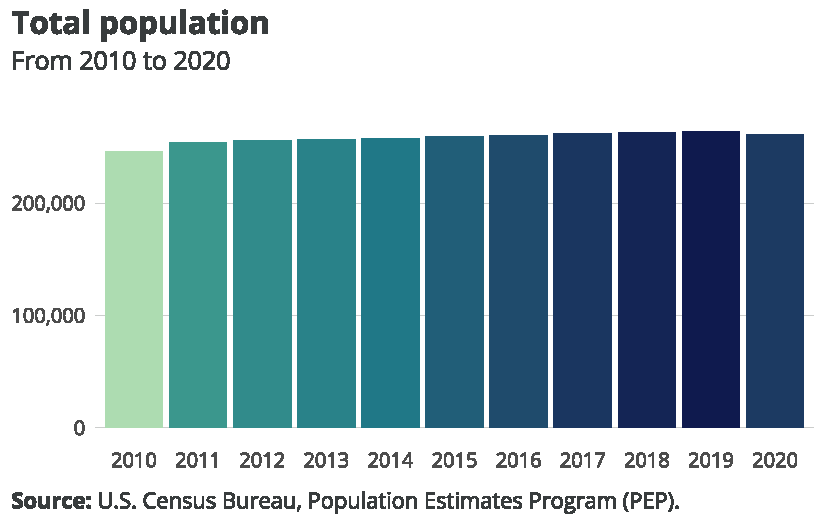
\includegraphics{./part-3-1_files/figure-pdf/fig-pop-1.pdf}

}

\caption{\label{fig-pop}Total regional population}

\end{figure}

\begin{figure}[H]

{\centering 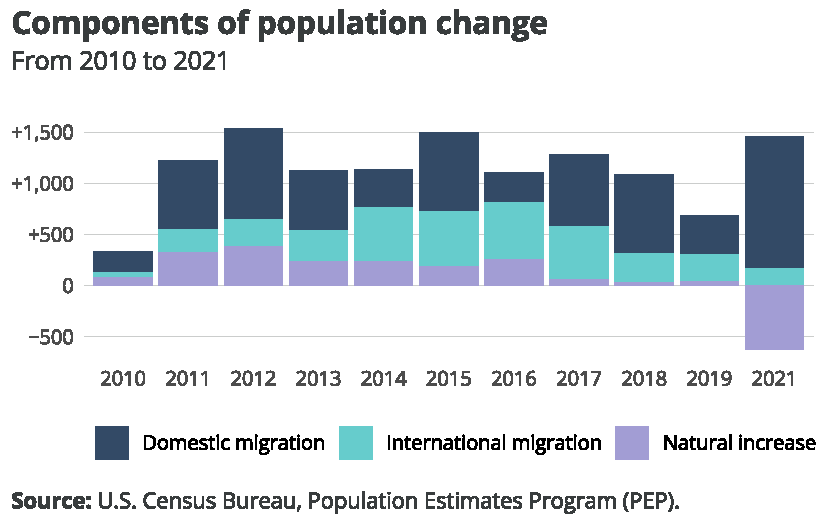
\includegraphics{./part-3-1_files/figure-pdf/fig-pchange-1.pdf}

}

\caption{\label{fig-pchange}Regional components of population change}

\end{figure}

\begin{figure}[H]

{\centering 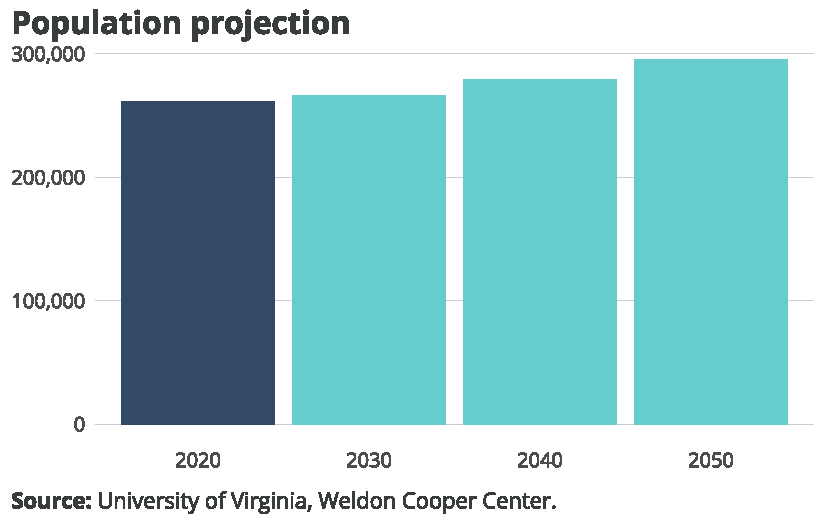
\includegraphics{./part-3-1_files/figure-pdf/fig-projections-1.pdf}

}

\caption{\label{fig-projections}Regional population projections}

\end{figure}

\hypertarget{household-trends}{%
\section{Household trends}\label{household-trends}}

\begin{figure}[H]

{\centering 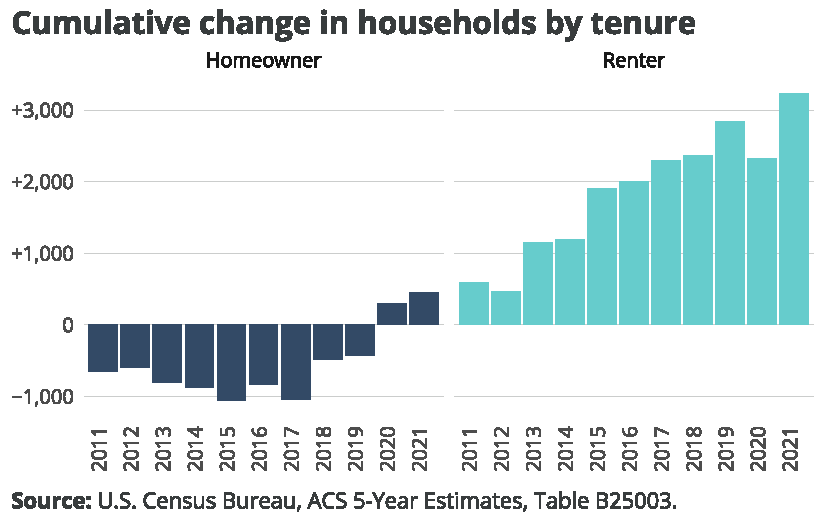
\includegraphics{./part-3-1_files/figure-pdf/fig-tenure-1.pdf}

}

\caption{\label{fig-tenure}Regional change in household tenure}

\end{figure}

\begin{figure}[H]

{\centering 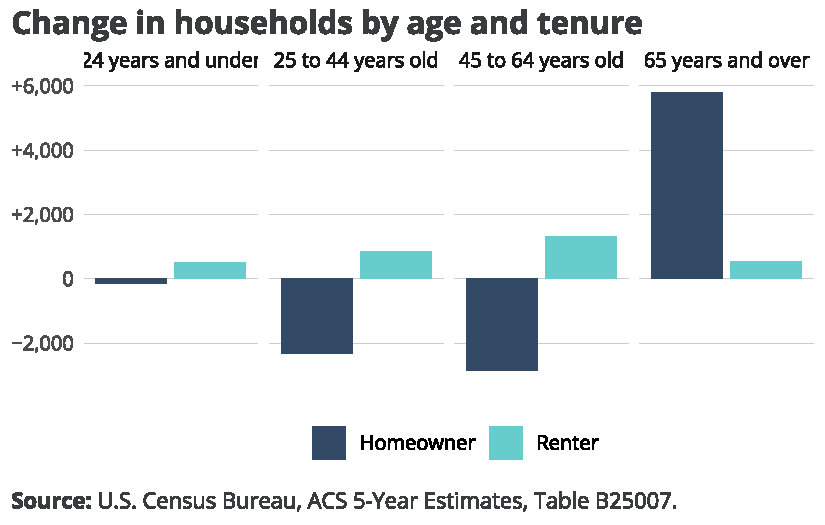
\includegraphics{./part-3-1_files/figure-pdf/fig-age-1.pdf}

}

\caption{\label{fig-age}Regional change in households by age and tenure}

\end{figure}

\begin{figure}[H]

{\centering 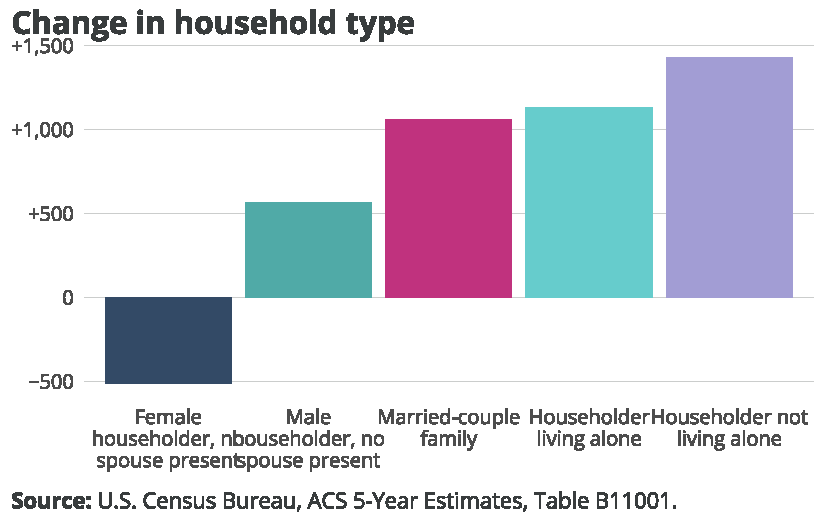
\includegraphics{./part-3-1_files/figure-pdf/fig-hhtype-1.pdf}

}

\caption{\label{fig-hhtype}Regional change in households by type}

\end{figure}

\begin{figure}[H]

{\centering 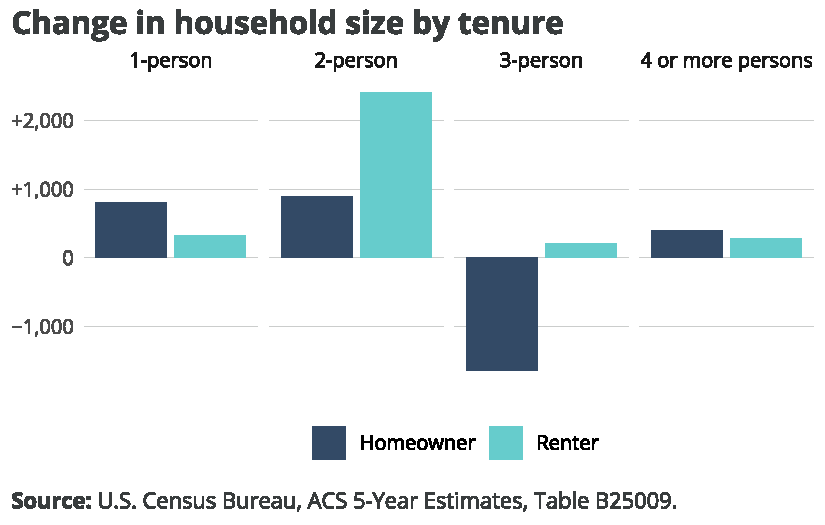
\includegraphics{./part-3-1_files/figure-pdf/fig-hhsize-1.pdf}

}

\caption{\label{fig-hhsize}Regional change in households by size and
tenure}

\end{figure}

\begin{figure}[H]

{\centering 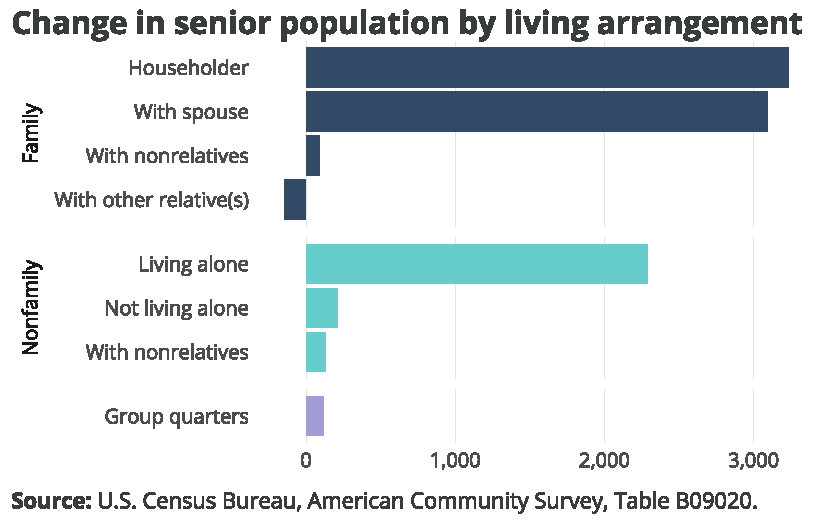
\includegraphics{./part-3-1_files/figure-pdf/fig-seniors-1.pdf}

}

\caption{\label{fig-seniors}Regional change in senior population}

\end{figure}

\begin{figure}[H]

{\centering 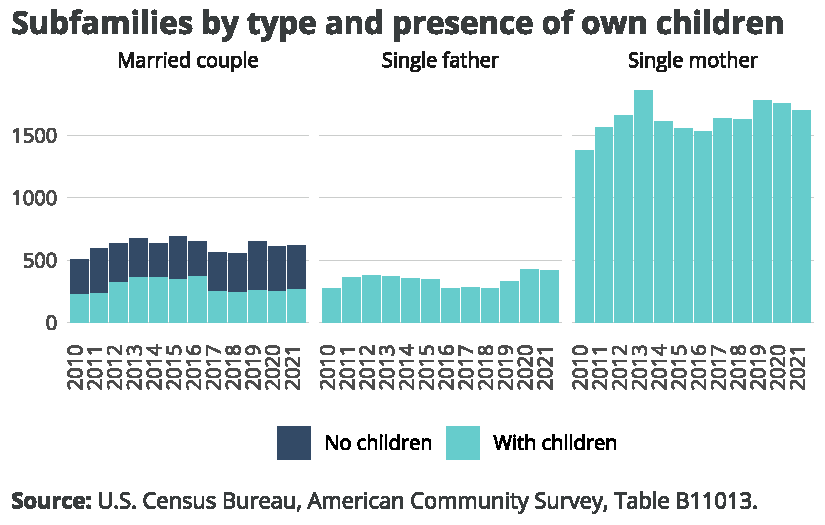
\includegraphics{./part-3-1_files/figure-pdf/fig-subfam-1.pdf}

}

\caption{\label{fig-subfam}Regional change in families living with
others}

\end{figure}

\begin{figure}[H]

{\centering 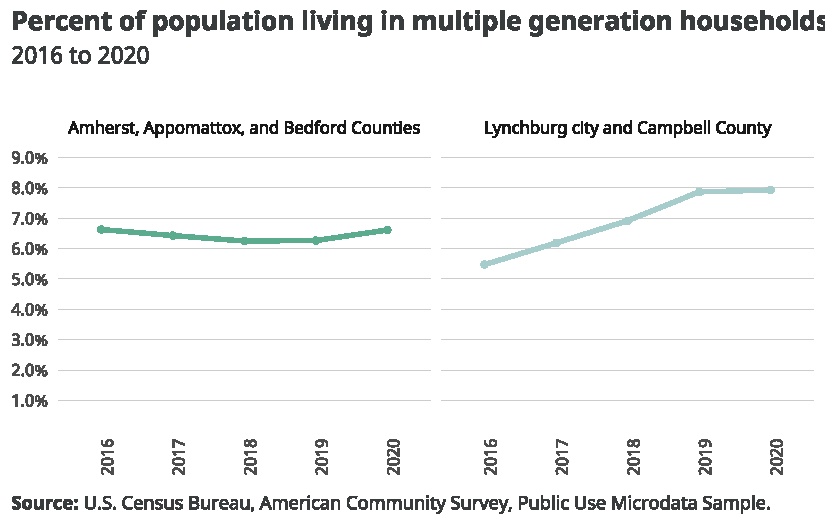
\includegraphics{./part-3-1_files/figure-pdf/fig-multigen-1.pdf}

}

\caption{\label{fig-multigen}Regional percentage of multigenerational
households}

\end{figure}

\begin{figure}[H]

{\centering 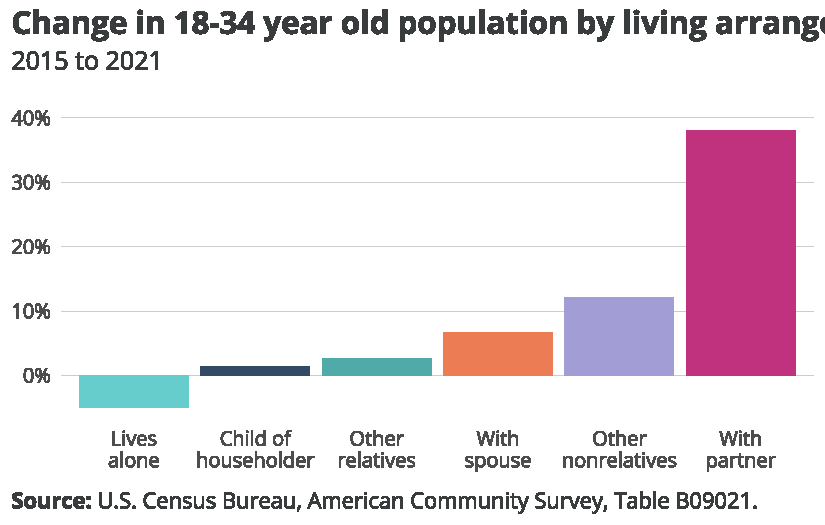
\includegraphics{./part-3-1_files/figure-pdf/fig-adultchild-1.pdf}

}

\caption{\label{fig-adultchild}Regional change in young adult population
by living arrangement}

\end{figure}

\hypertarget{economic-trends}{%
\section{Economic trends}\label{economic-trends}}

\begin{figure}[H]

{\centering 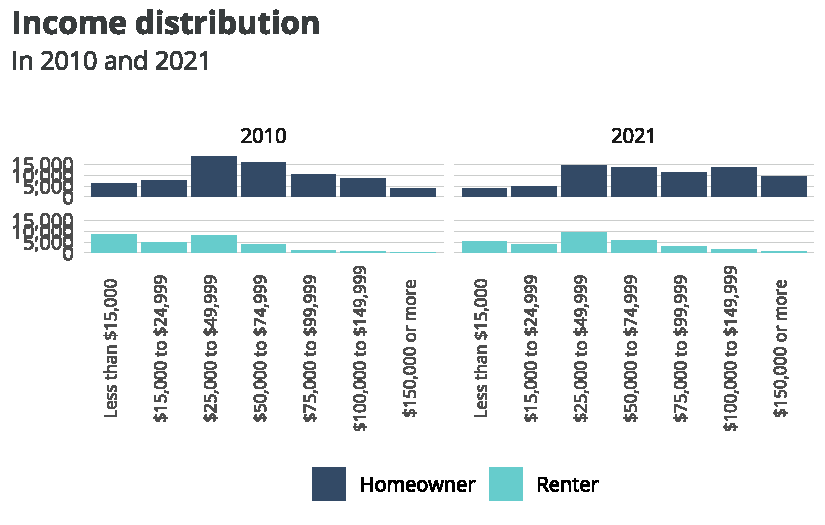
\includegraphics{./part-3-1_files/figure-pdf/fig-incdist-1.pdf}

}

\caption{\label{fig-incdist}Regional income distribution by tenure}

\end{figure}

\begin{figure}[H]

{\centering 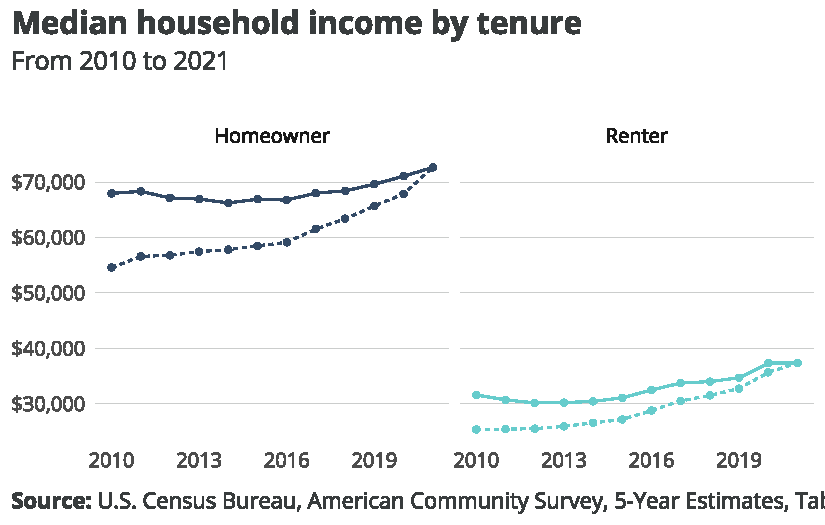
\includegraphics{./part-3-1_files/figure-pdf/fig-medinc-1.pdf}

}

\caption{\label{fig-medinc}Regional median household income by tenure}

\end{figure}

\begin{figure}[H]

{\centering 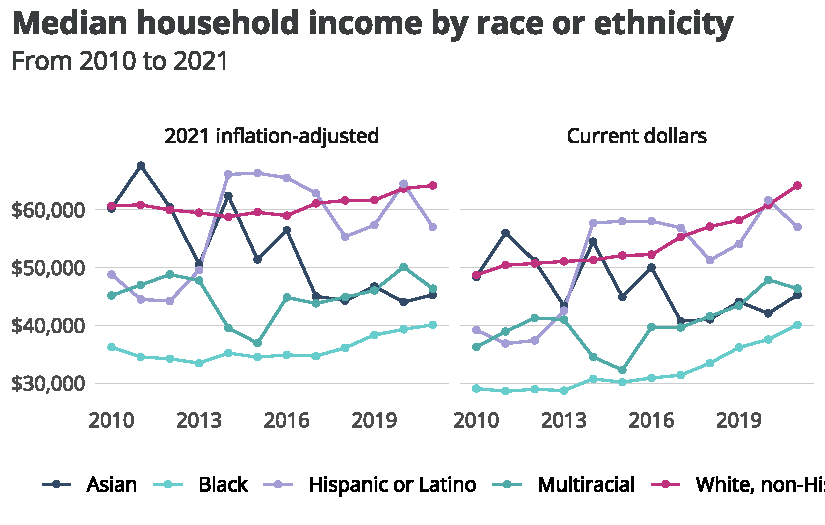
\includegraphics{./part-3-1_files/figure-pdf/fig-inc-race-msa-1.pdf}

}

\caption{\label{fig-inc-race-msa}Regional median household income by
race and ethnicity}

\end{figure}

\hypertarget{housing-stock}{%
\section{Housing stock}\label{housing-stock}}

\begin{figure}[H]

{\centering 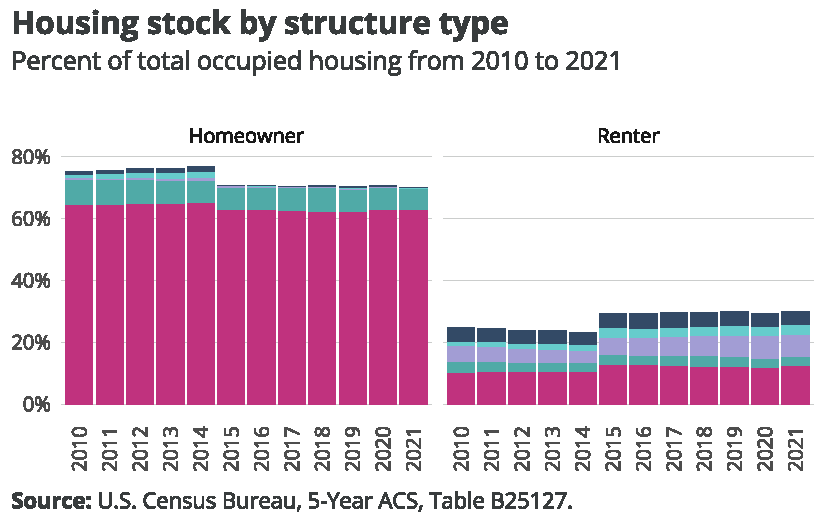
\includegraphics{./part-3-1_files/figure-pdf/fig-structure-1.pdf}

}

\caption{\label{fig-structure}Regional housing stock by structure type}

\end{figure}

\begin{figure}[H]

{\centering 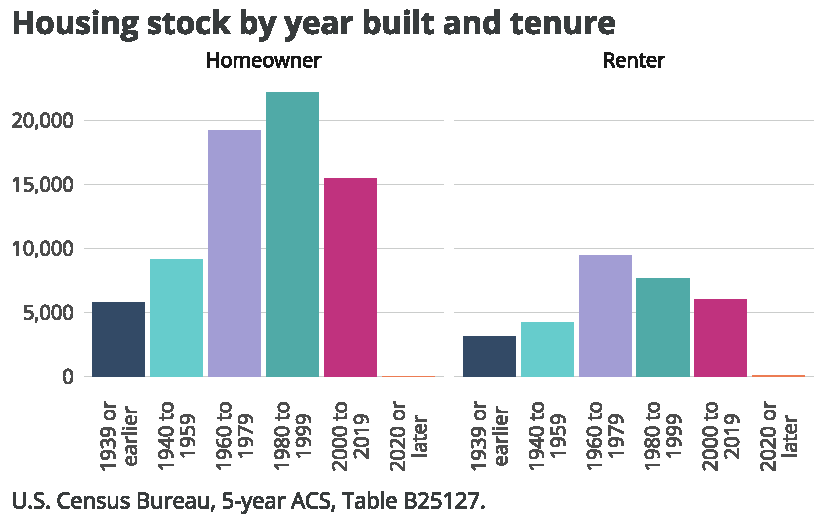
\includegraphics{./part-3-1_files/figure-pdf/fig-yrbuilt-1.pdf}

}

\caption{\label{fig-yrbuilt}Regional housing stock by year built}

\end{figure}

\begin{figure}[H]

{\centering 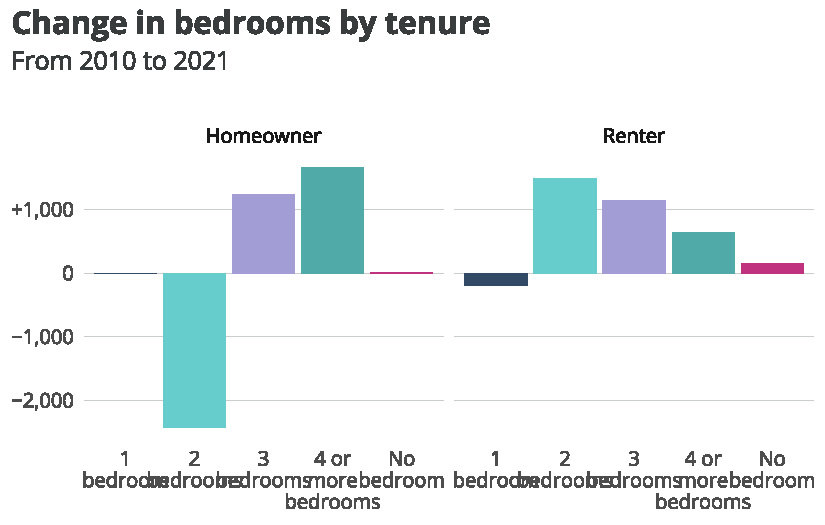
\includegraphics{./part-3-1_files/figure-pdf/fig-beds-1.pdf}

}

\caption{\label{fig-beds}Change in regional housing stock by bedroom
count}

\end{figure}

\begin{figure}[H]

{\centering 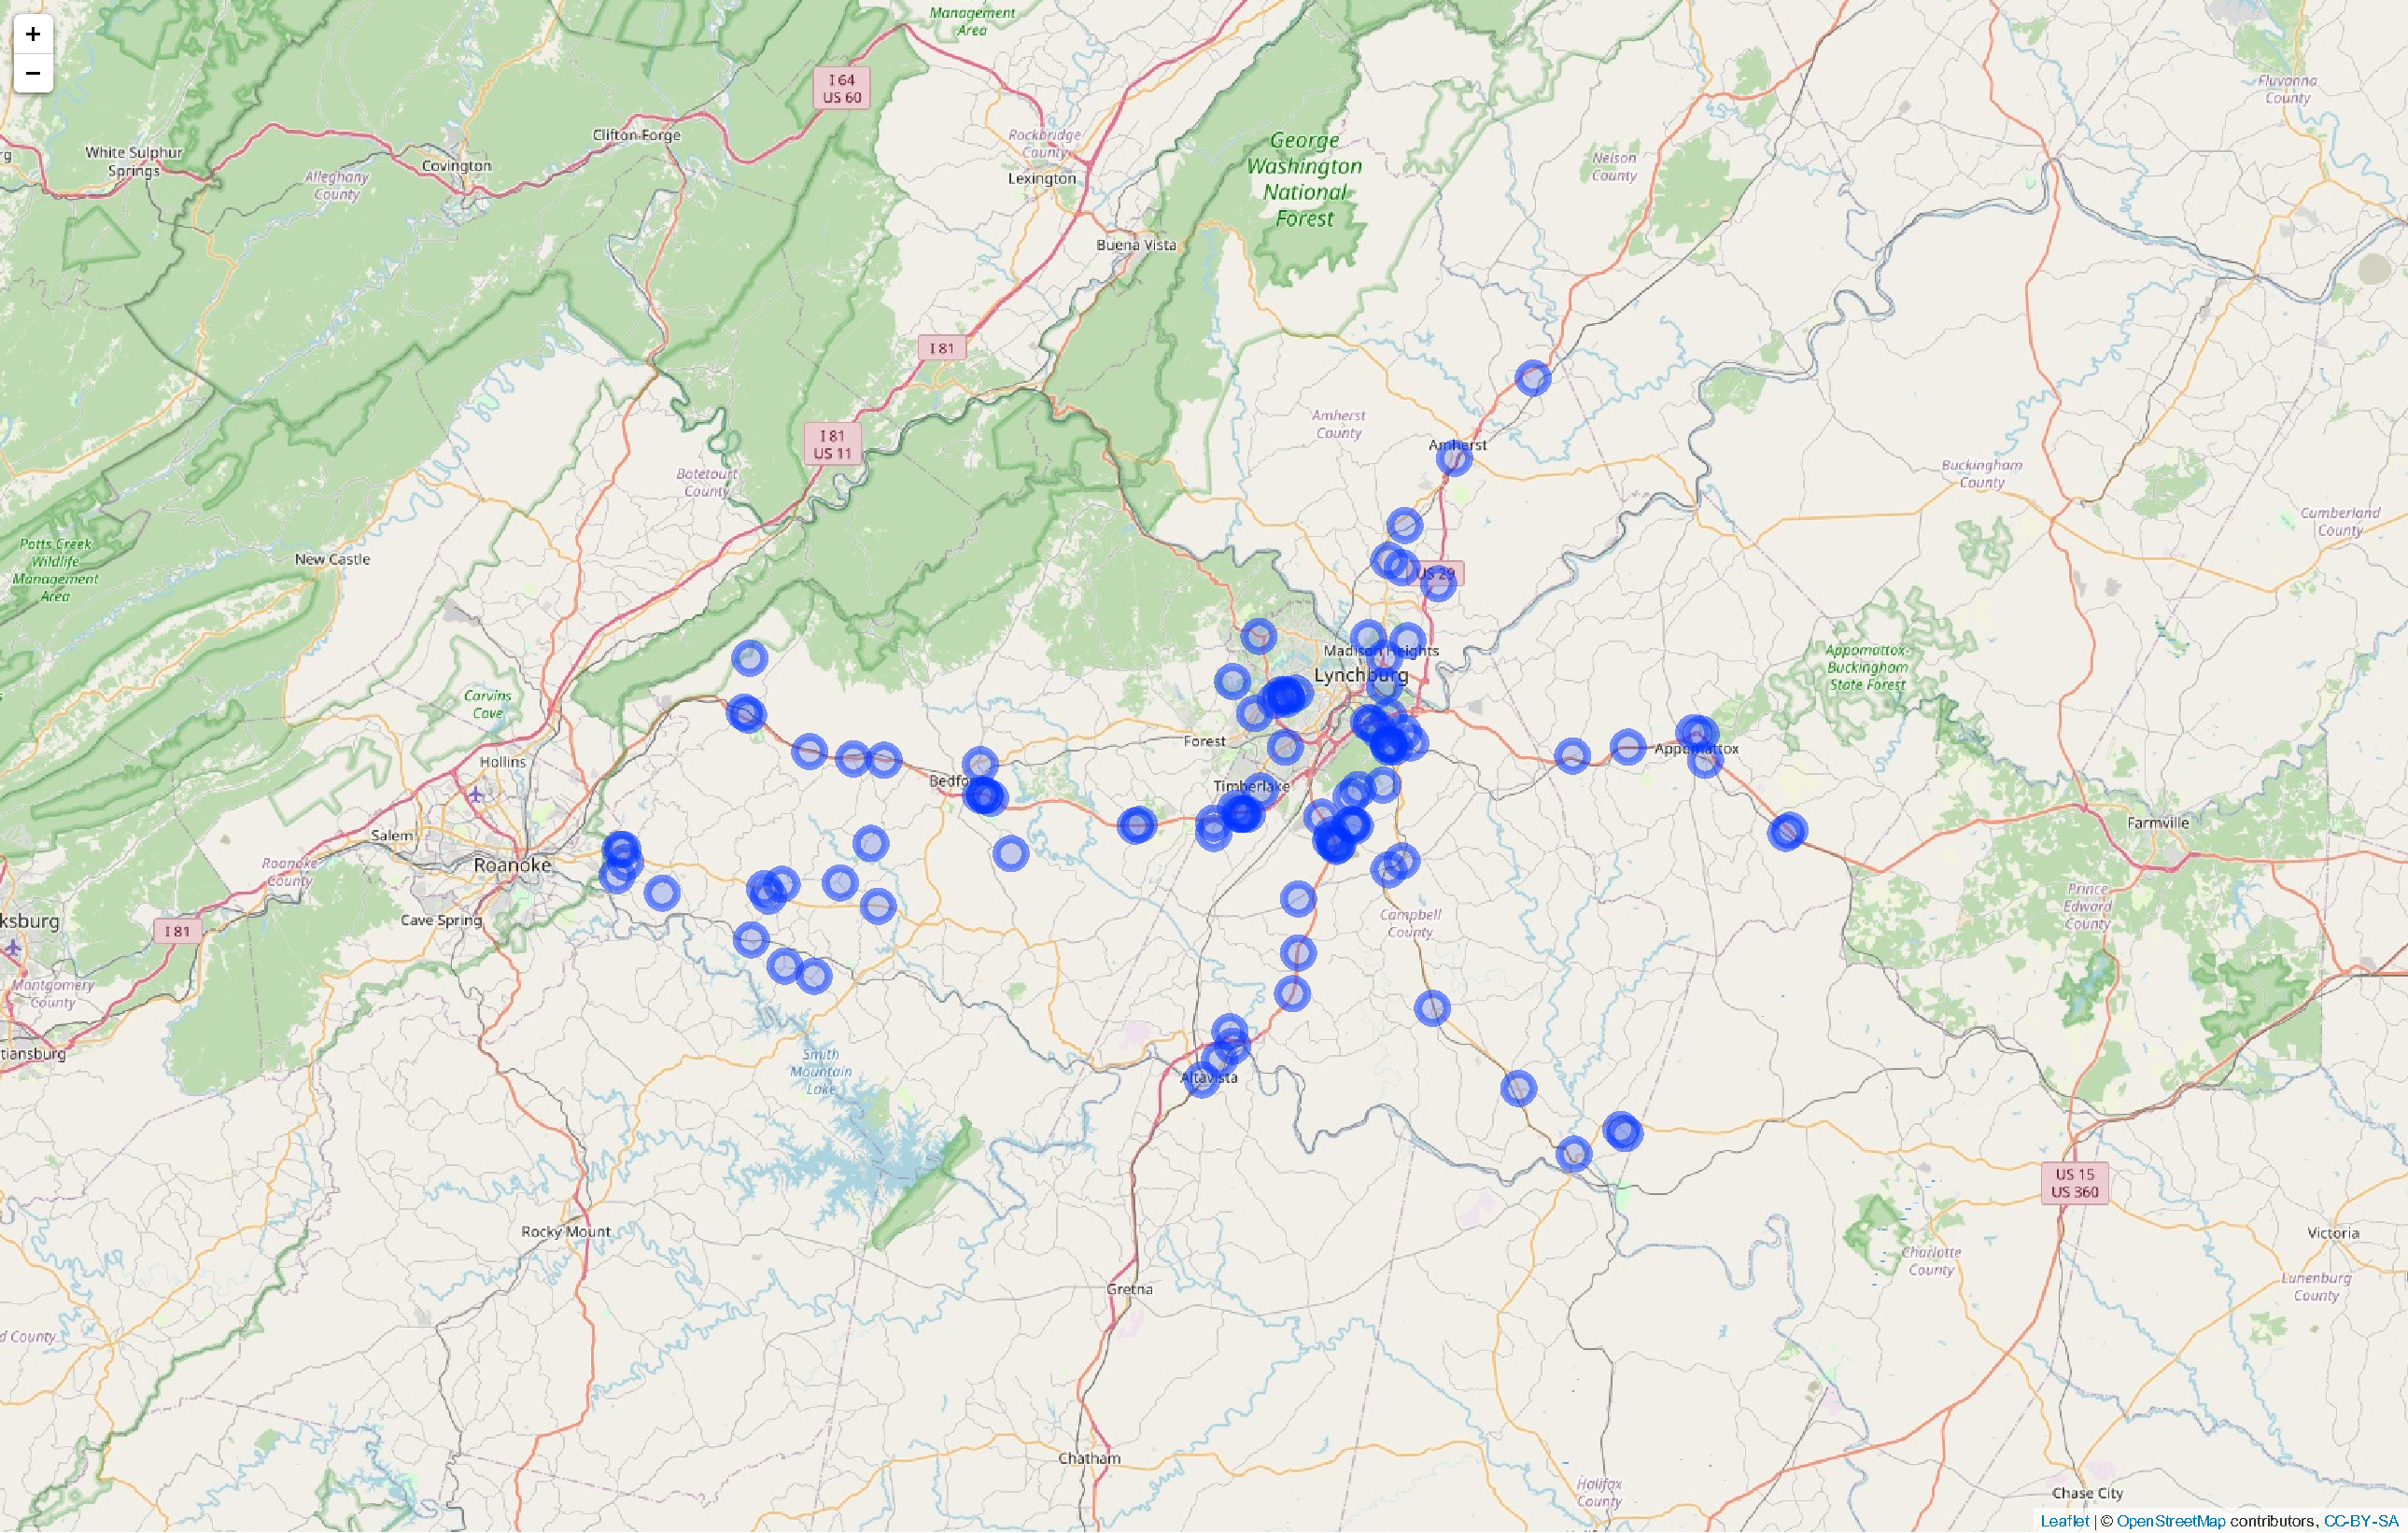
\includegraphics{./part-3-1_files/figure-pdf/fig-mhc-map-1.pdf}

}

\caption{\label{fig-mhc-map}Map of manufactured home communities}

\end{figure}

\begin{figure}[H]

{\centering 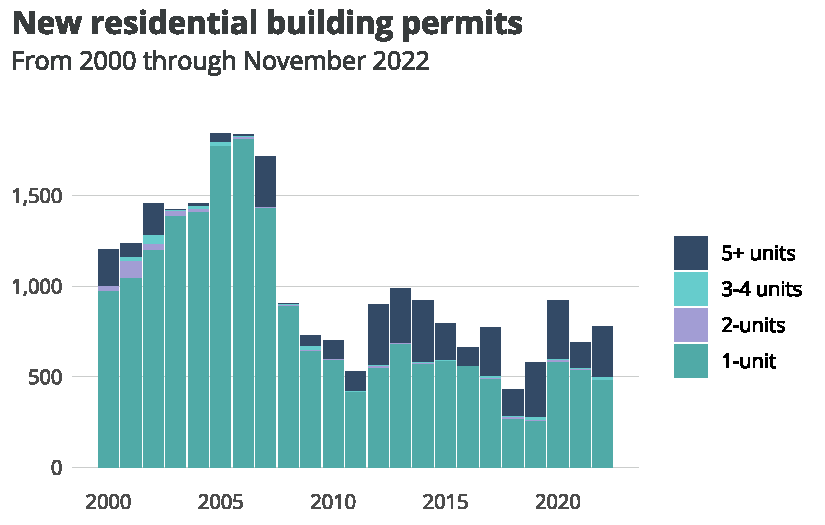
\includegraphics{./part-3-1_files/figure-pdf/fig-permits-1.pdf}

}

\caption{\label{fig-permits}Regional residential building permits}

\end{figure}

\hypertarget{homeownership-market}{%
\section{Homeownership market}\label{homeownership-market}}

\begin{figure}[H]

{\centering 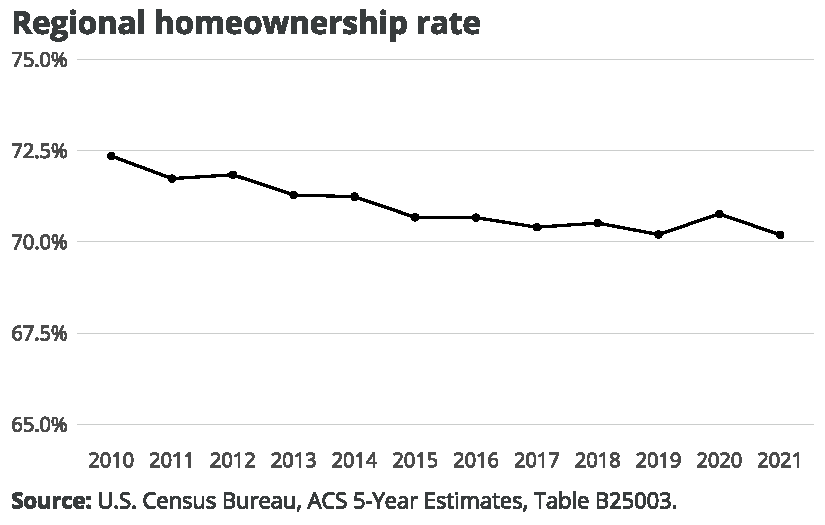
\includegraphics{./part-3-1_files/figure-pdf/fig-ho-rate-1.pdf}

}

\caption{\label{fig-ho-rate}Regional homeownership rate}

\end{figure}

\begin{figure}[H]

{\centering 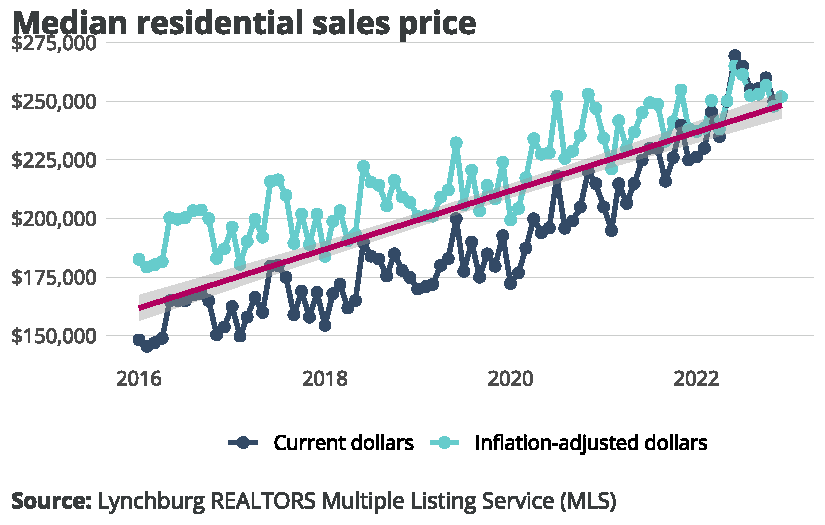
\includegraphics{./part-3-1_files/figure-pdf/fig-mls-price-1.pdf}

}

\caption{\label{fig-mls-price}Regional median residential sales price}

\end{figure}

\begin{figure}[H]

{\centering 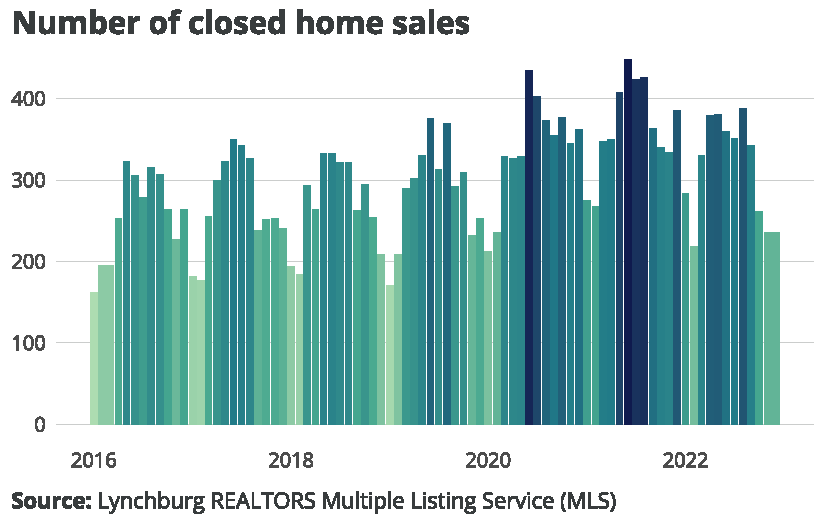
\includegraphics{./part-3-1_files/figure-pdf/fig-mls-sales-1.pdf}

}

\caption{\label{fig-mls-sales}Regional number of closed home sales}

\end{figure}

\begin{figure}[H]

{\centering 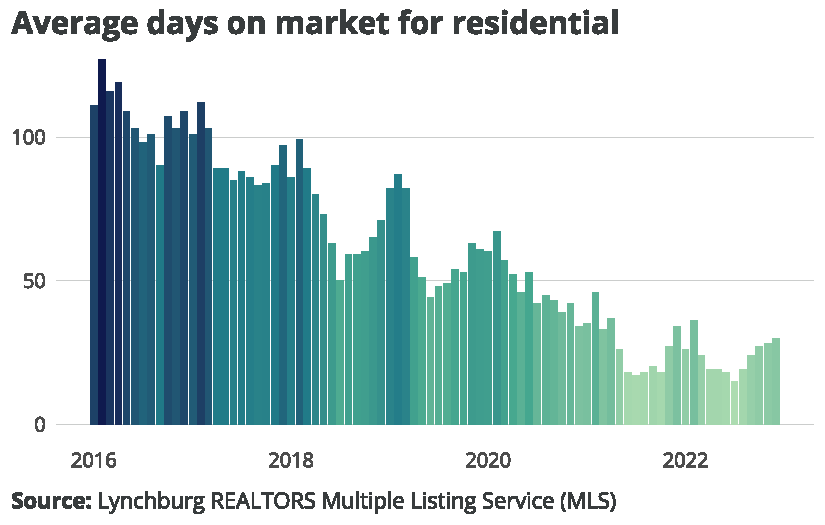
\includegraphics{./part-3-1_files/figure-pdf/fig-mls-dom-1.pdf}

}

\caption{\label{fig-mls-dom}Regional average days on market}

\end{figure}

\hypertarget{rental-market}{%
\section{Rental market}\label{rental-market}}

\begin{figure}[H]

{\centering 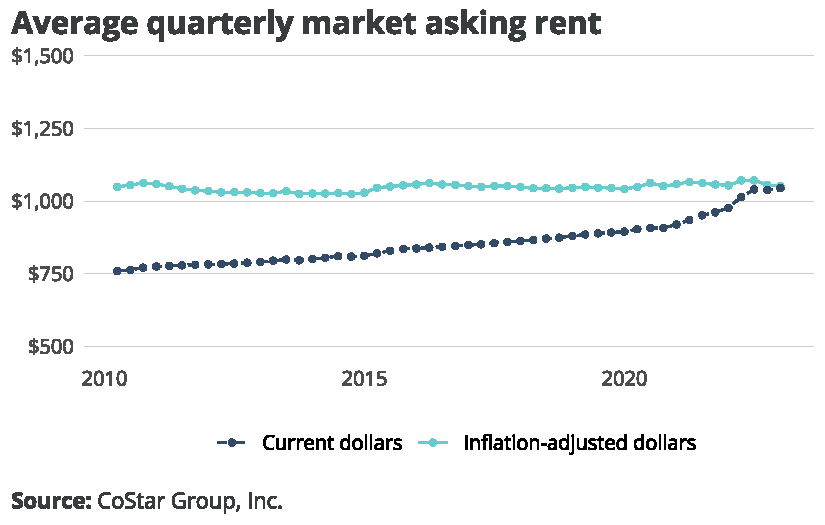
\includegraphics{./part-3-1_files/figure-pdf/fig-rent-1.pdf}

}

\caption{\label{fig-rent}Regional average market asking rent}

\end{figure}

\begin{figure}[H]

{\centering 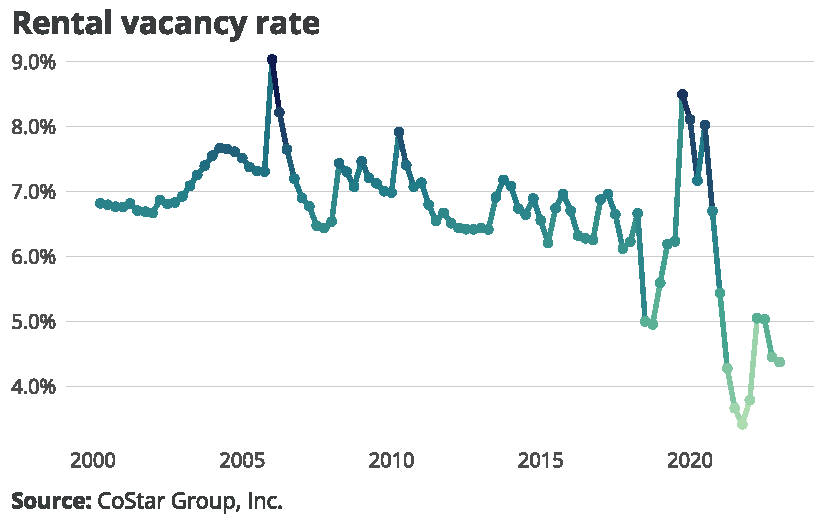
\includegraphics{./part-3-1_files/figure-pdf/fig-vacancy-1.pdf}

}

\caption{\label{fig-vacancy}Regional rental vacancy rate}

\end{figure}

\hypertarget{affordability}{%
\section{Affordability}\label{affordability}}

\begin{figure}[H]

{\centering 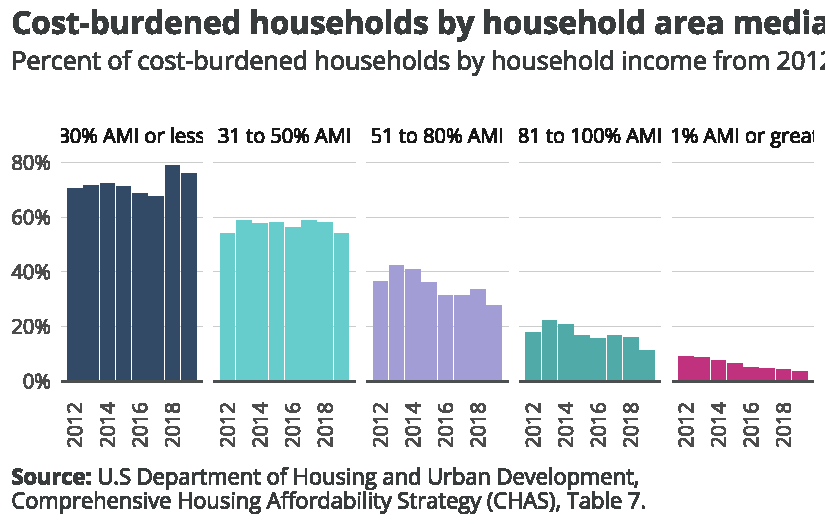
\includegraphics{./part-3-1_files/figure-pdf/fig-cb-total-1.pdf}

}

\caption{\label{fig-cb-total}Total regional housing cost burden by
household area median income}

\end{figure}

\begin{figure}[H]

{\centering 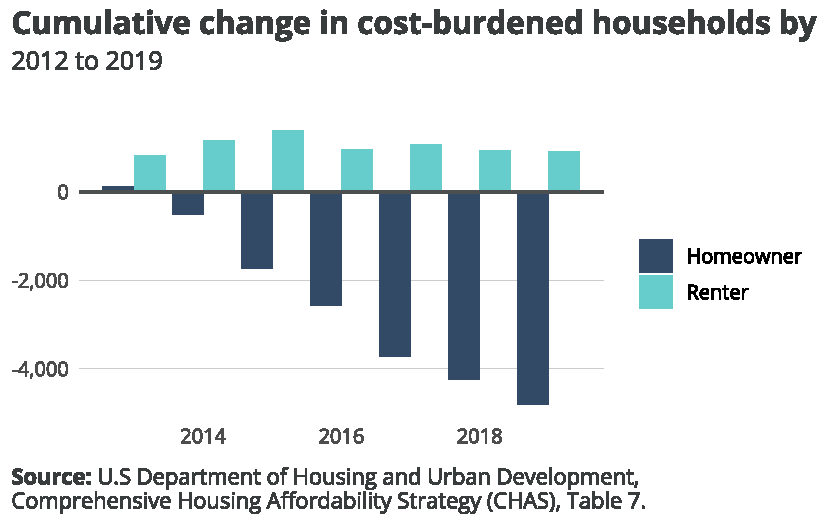
\includegraphics{./part-3-1_files/figure-pdf/fig-cb-change-1.pdf}

}

\caption{\label{fig-cb-change}Regional change in cost-burdened
households by tenure}

\end{figure}

\begin{figure}[H]

{\centering 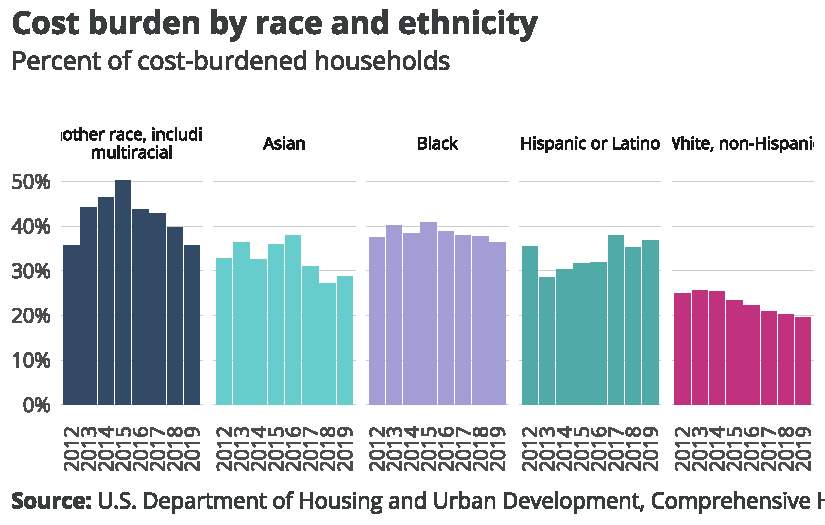
\includegraphics{./part-3-1_files/figure-pdf/fig-cb-race-1.pdf}

}

\caption{\label{fig-cb-race}Regional percent of cost-burdened households
by race and ethnicity}

\end{figure}

\begin{figure}[H]

{\centering 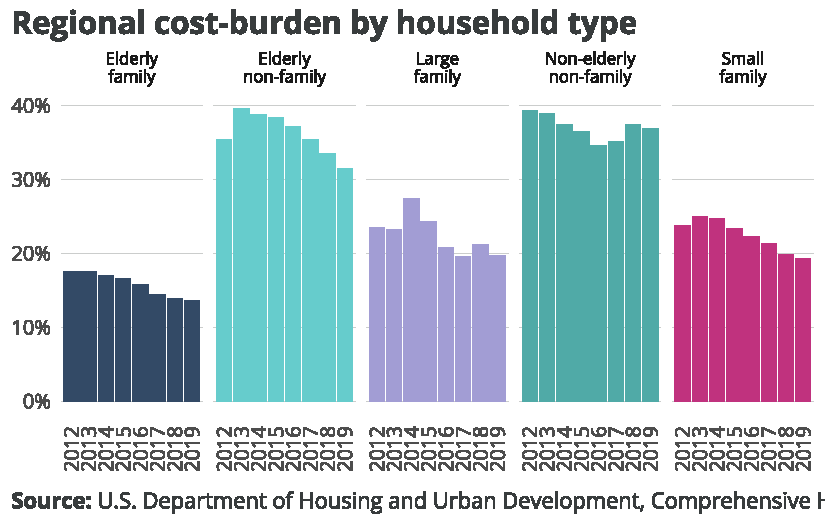
\includegraphics{./part-3-1_files/figure-pdf/fig-hh-cb-1.pdf}

}

\caption{\label{fig-hh-cb}Regional cost-burden by household type}

\end{figure}

\hypertarget{county-housing-market-assessment}{%
\chapter{County Housing Market
Assessment}\label{county-housing-market-assessment}}

The following provides a county-level analysis of major trends impacting
housing within Central Virginia Planning District region. All data has
been disaggregated to show the differences between localities.

\hypertarget{takeaways-1}{%
\section{Takeaways}\label{takeaways-1}}

\hypertarget{population-trends-1}{%
\section{Population trends}\label{population-trends-1}}

\begin{figure}[H]

{\centering 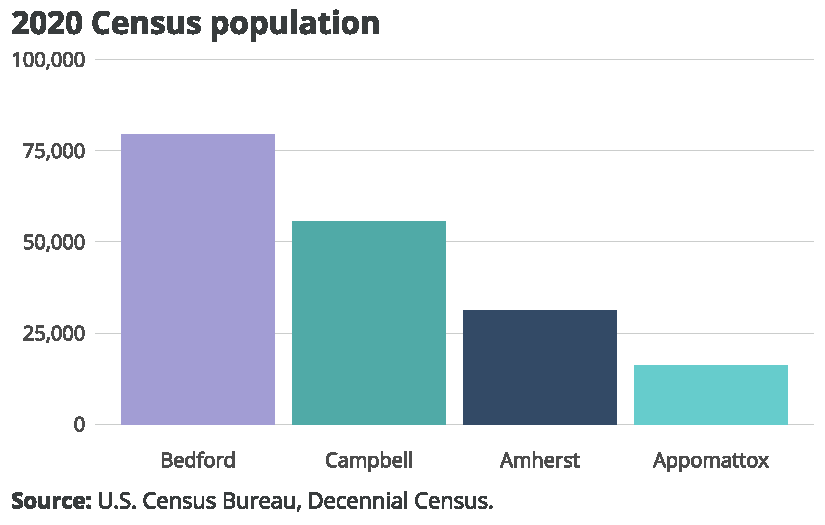
\includegraphics{./part-3-2_files/figure-pdf/fig-localpop-1.pdf}

}

\caption{\label{fig-localpop}2020 Census population by county}

\end{figure}

\begin{figure}[H]

{\centering 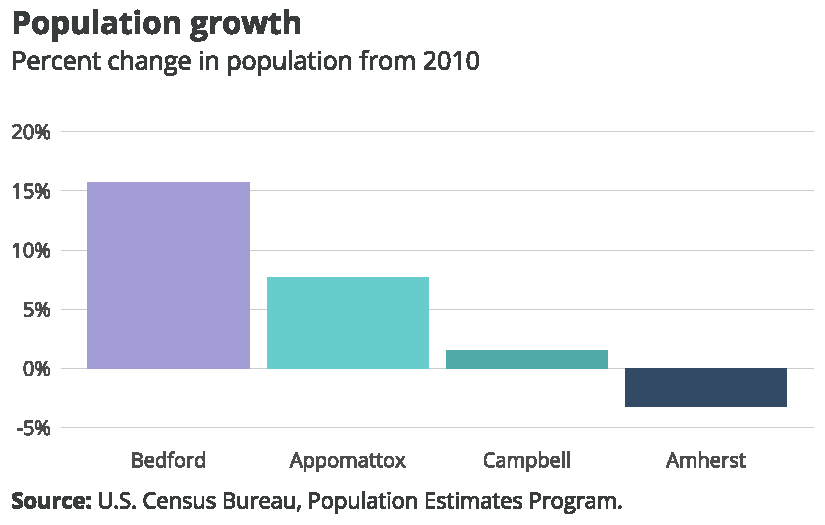
\includegraphics{./part-3-2_files/figure-pdf/fig-local-pchg-1.pdf}

}

\caption{\label{fig-local-pchg}Population growth by county}

\end{figure}

\begin{figure}[H]

{\centering 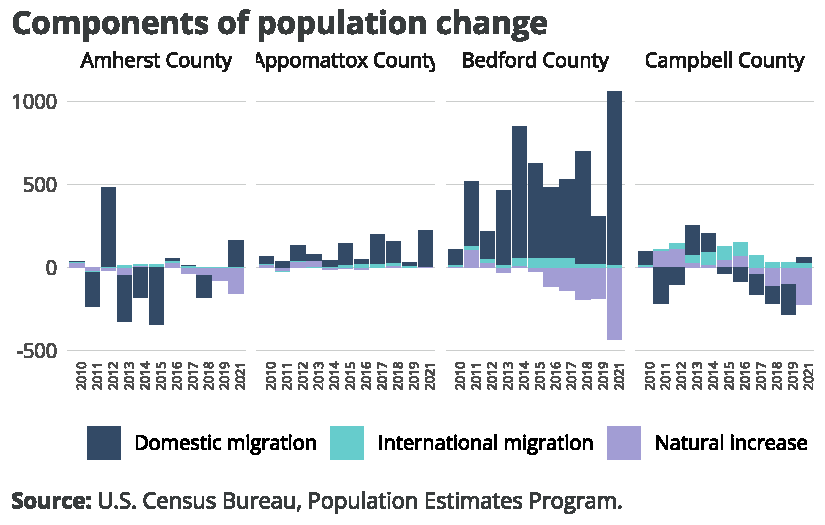
\includegraphics{./part-3-2_files/figure-pdf/fig-local-chg-1.pdf}

}

\caption{\label{fig-local-chg}Components of population change by county}

\end{figure}

\begin{figure}[H]

{\centering 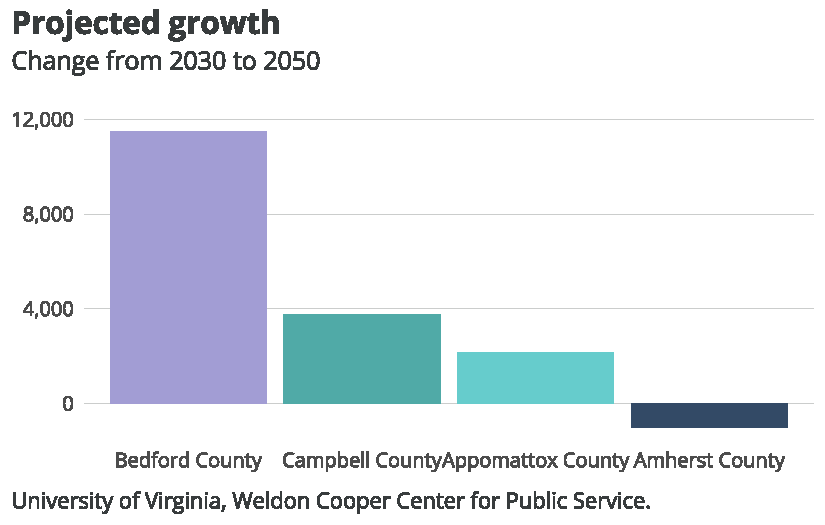
\includegraphics{./part-3-2_files/figure-pdf/fig-localproj-1.pdf}

}

\caption{\label{fig-localproj}Projected population growth 2030 to 2050
by county}

\end{figure}

\hypertarget{household-trends-1}{%
\section{Household trends}\label{household-trends-1}}

\begin{figure}[H]

{\centering 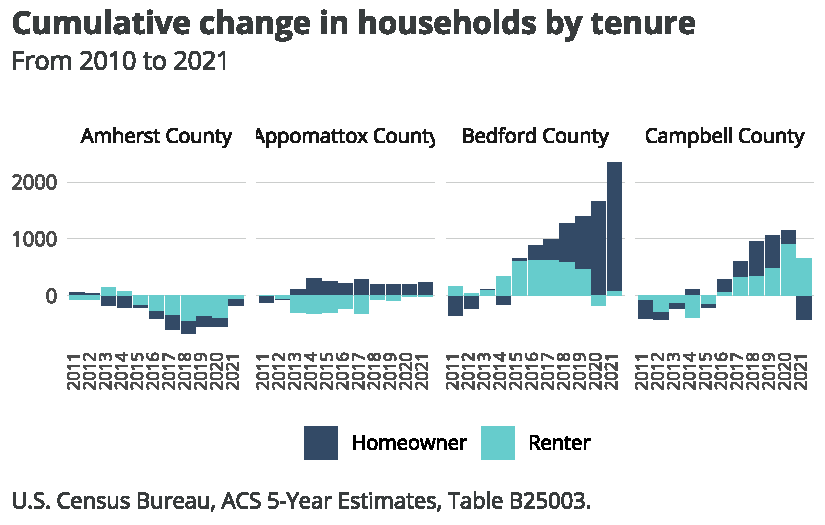
\includegraphics{./part-3-2_files/figure-pdf/fig-localtenure-1.pdf}

}

\caption{\label{fig-localtenure}Local cumulative change in households by
tenure}

\end{figure}

\begin{figure}[H]

{\centering 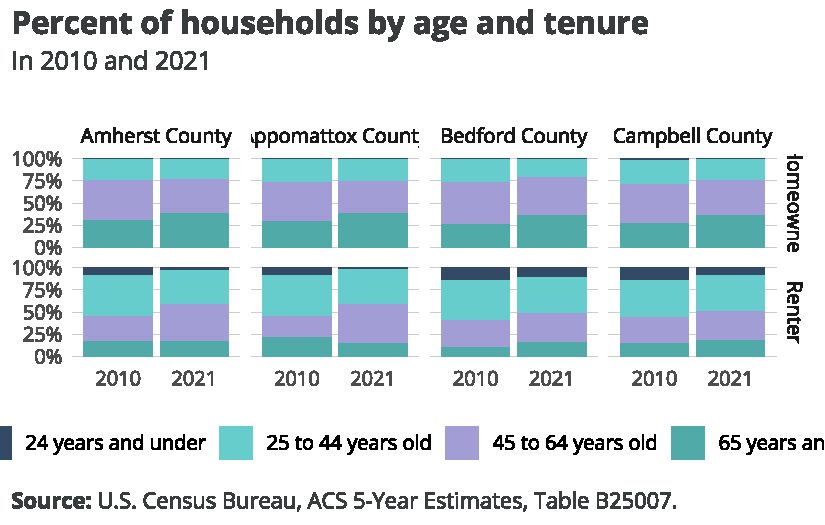
\includegraphics{./part-3-2_files/figure-pdf/fig-localage-1.pdf}

}

\caption{\label{fig-localage}Local percent of households by age and
tenure}

\end{figure}

\begin{figure}[H]

{\centering 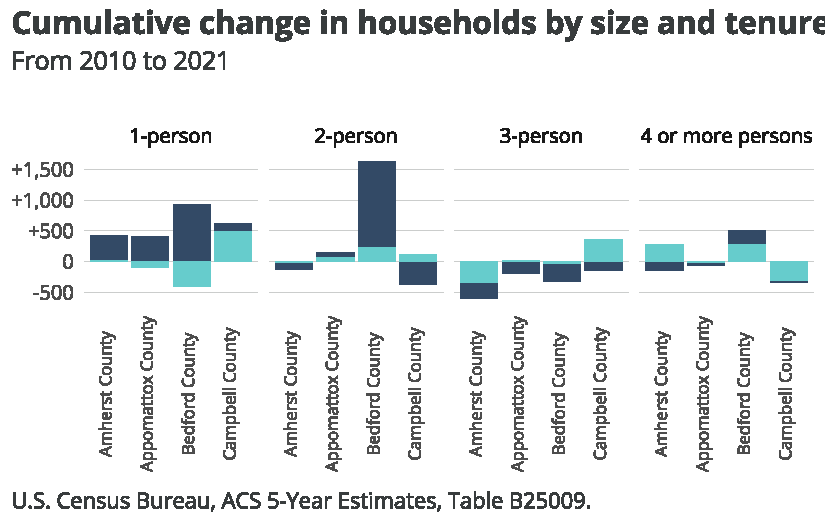
\includegraphics{./part-3-2_files/figure-pdf/fig-localsize-1.pdf}

}

\caption{\label{fig-localsize}Local cumulative change in households by
size and tenure}

\end{figure}

\begin{figure}[H]

{\centering 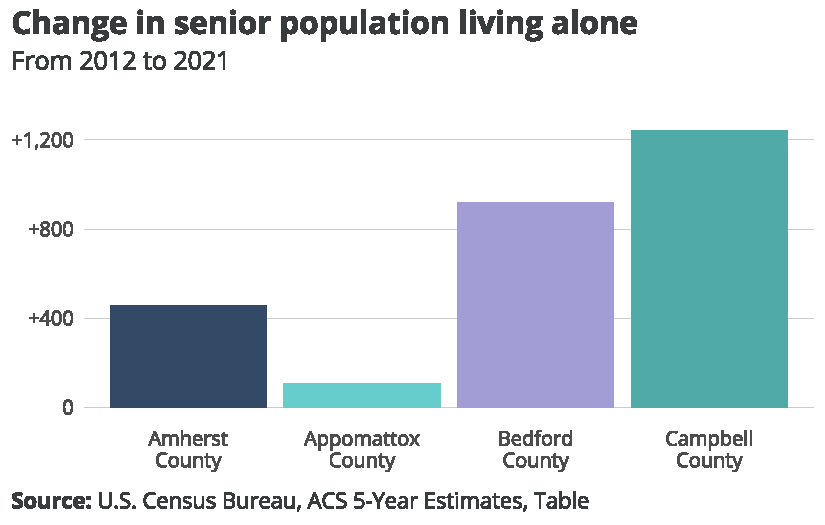
\includegraphics{./part-3-2_files/figure-pdf/fig-localsenior-1.pdf}

}

\caption{\label{fig-localsenior}Local change in senior population living
alone}

\end{figure}

\begin{figure}[H]

{\centering 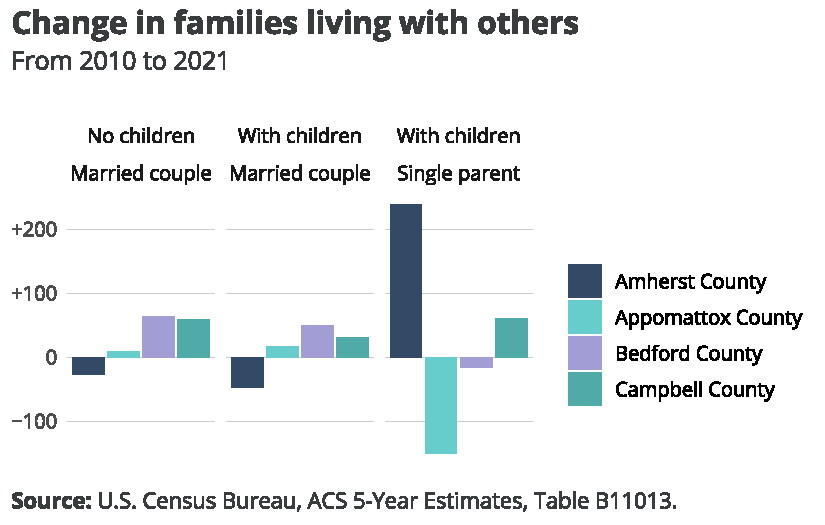
\includegraphics{./part-3-2_files/figure-pdf/fig-localsubfam-1.pdf}

}

\caption{\label{fig-localsubfam}Local change in families living with
others}

\end{figure}

\begin{figure}[H]

{\centering 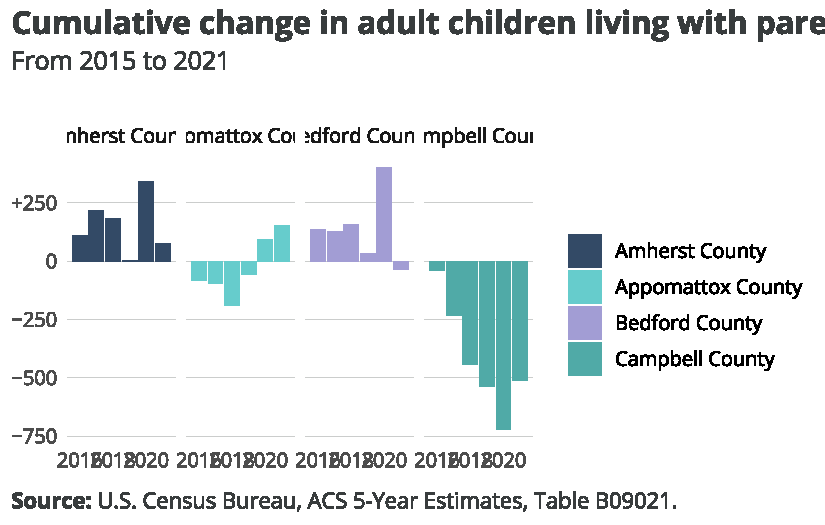
\includegraphics{./part-3-2_files/figure-pdf/fig-localachild-1.pdf}

}

\caption{\label{fig-localachild}Local cumulative change in adult
children living with parents}

\end{figure}

\hypertarget{economic-trends-1}{%
\section{Economic trends}\label{economic-trends-1}}

\begin{figure}[H]

{\centering 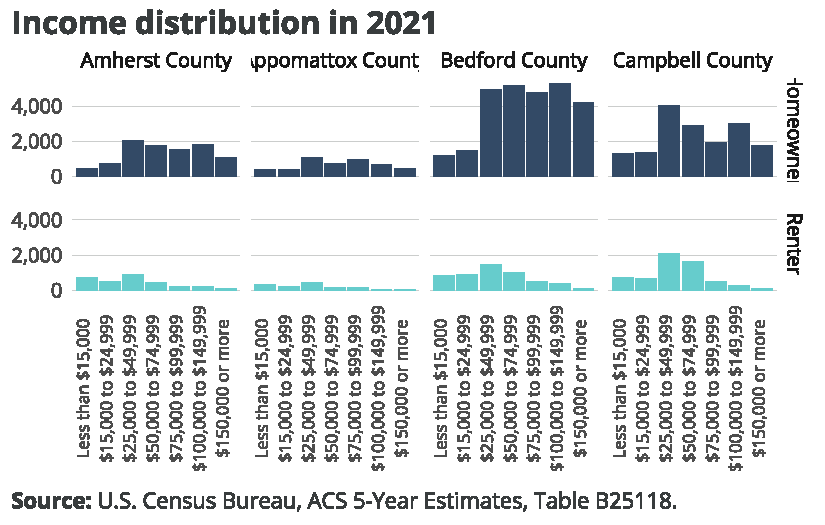
\includegraphics{./part-3-2_files/figure-pdf/fig-localinc-distribution-1.pdf}

}

\caption{\label{fig-localinc-distribution}Local income distribution by
tenure}

\end{figure}

\begin{figure}[H]

{\centering 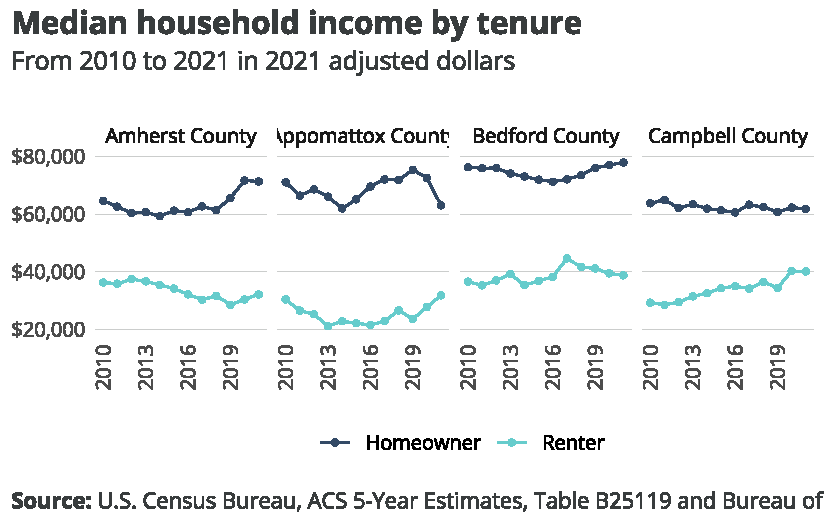
\includegraphics{./part-3-2_files/figure-pdf/fig-med-inc-1.pdf}

}

\caption{\label{fig-med-inc}Local median household income by tenure}

\end{figure}

\begin{figure}[H]

{\centering 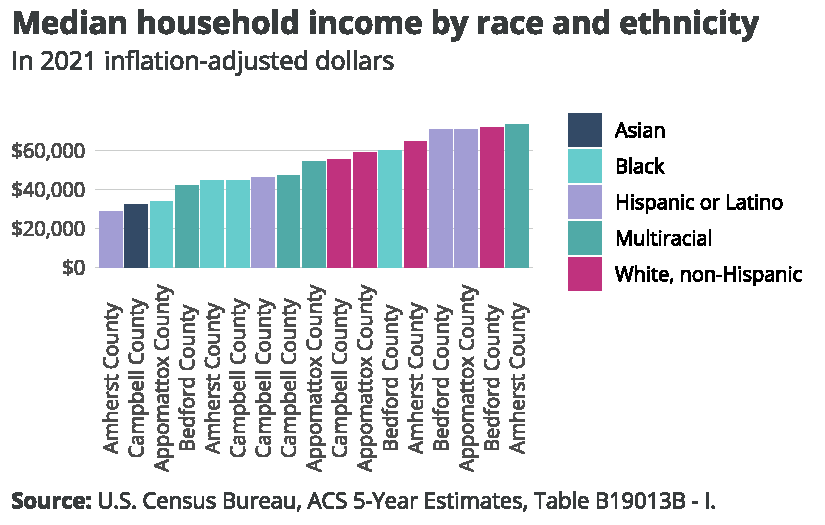
\includegraphics{./part-3-2_files/figure-pdf/fig-localrace-inc-1.pdf}

}

\caption{\label{fig-localrace-inc}Local median household income by race
and ethnicity}

\end{figure}

\hypertarget{housing-stock-1}{%
\section{Housing stock}\label{housing-stock-1}}

\begin{figure}[H]

{\centering 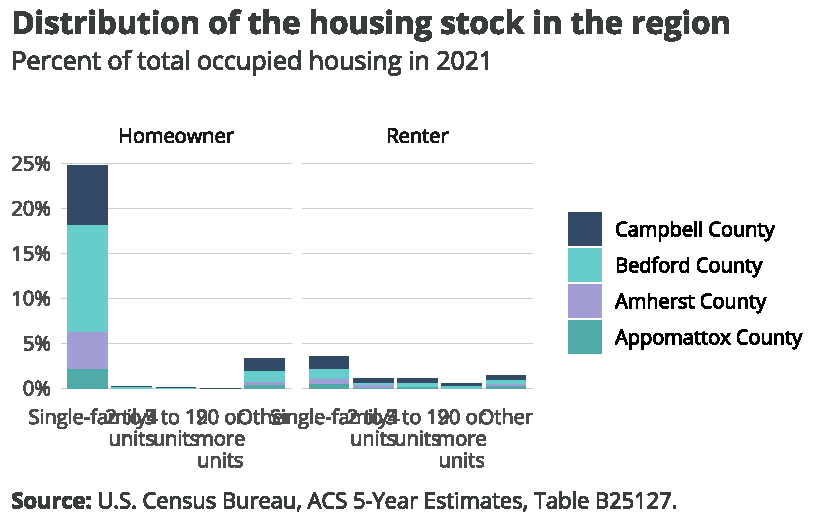
\includegraphics{./part-3-2_files/figure-pdf/fig-localstructure-1.pdf}

}

\caption{\label{fig-localstructure}Distribution of house stock in the
region}

\end{figure}

\begin{figure}[H]

{\centering 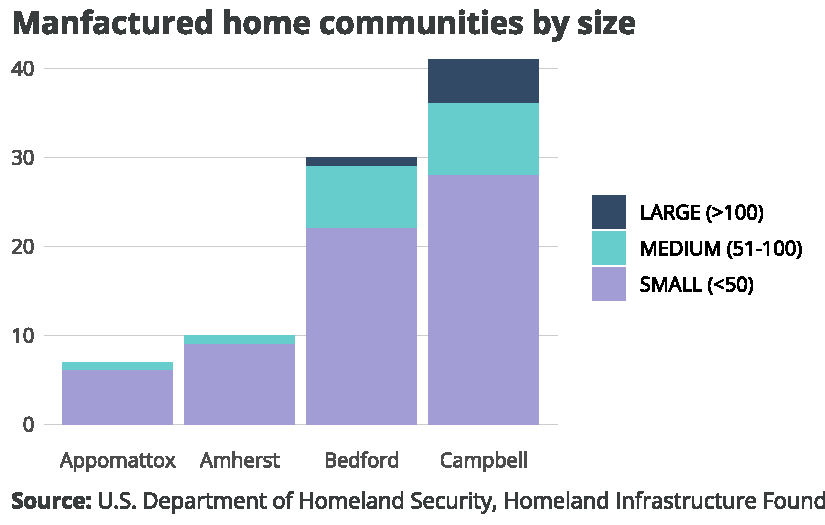
\includegraphics{./part-3-2_files/figure-pdf/fig-mhc-county-1.pdf}

}

\caption{\label{fig-mhc-county}Local manufactured home communities by
size}

\end{figure}

\begin{figure}[H]

{\centering 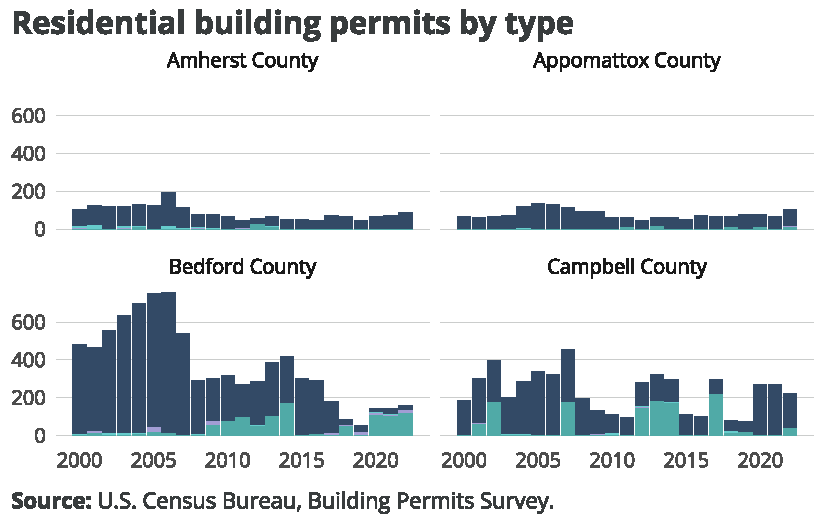
\includegraphics{./part-3-2_files/figure-pdf/fig-localbps-1.pdf}

}

\caption{\label{fig-localbps}Local esidential building permits by type}

\end{figure}

\hypertarget{homeownership-market-1}{%
\section{Homeownership market}\label{homeownership-market-1}}

\begin{figure}[H]

{\centering 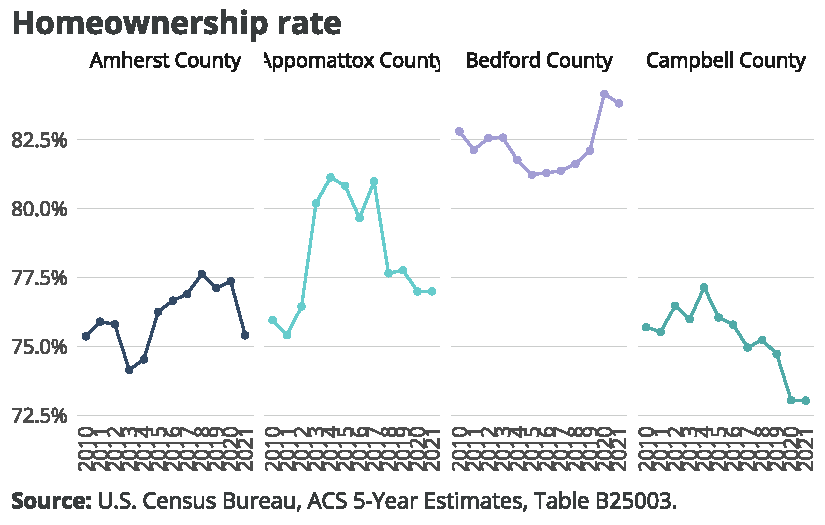
\includegraphics{./part-3-2_files/figure-pdf/fig-localho-1.pdf}

}

\caption{\label{fig-localho}Local homeownership rates}

\end{figure}

\hypertarget{rental-market-1}{%
\section{Rental market}\label{rental-market-1}}

\begin{figure}[H]

{\centering 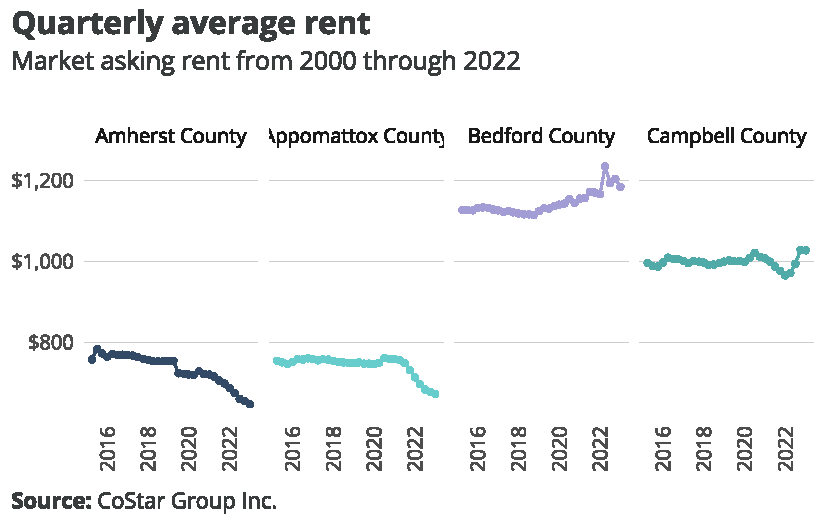
\includegraphics{./part-3-2_files/figure-pdf/fig-localrent-1.pdf}

}

\caption{\label{fig-localrent}Local quarterly average market asking
rents}

\end{figure}

\begin{figure}[H]

{\centering 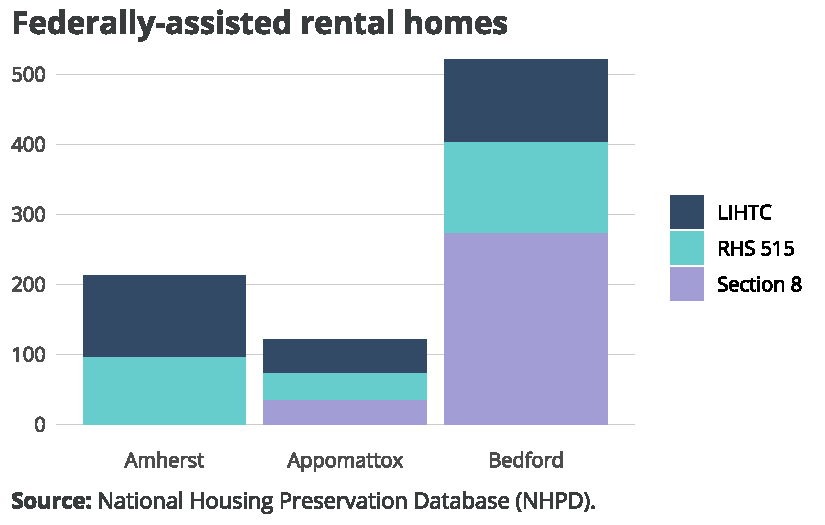
\includegraphics{./part-3-2_files/figure-pdf/fig-nhpd-1.pdf}

}

\caption{\label{fig-nhpd}Federally assisted rental homes by county}

\end{figure}

\begin{figure}[H]

{\centering 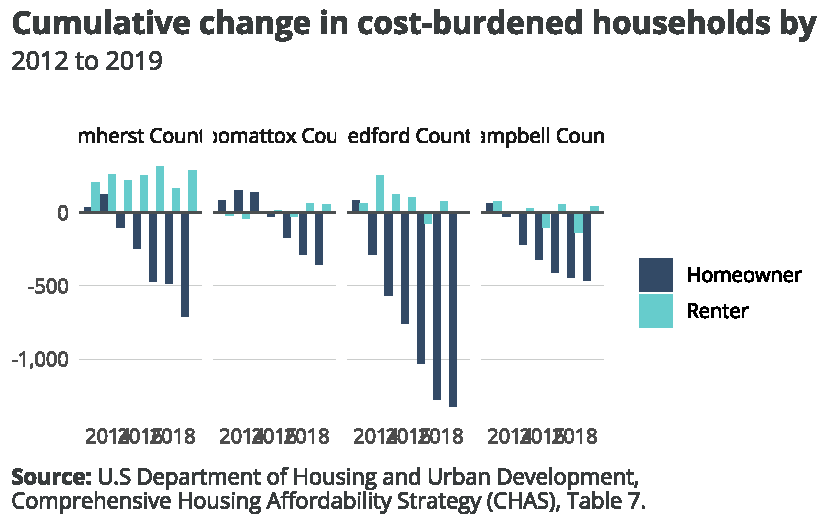
\includegraphics{./part-3-2_files/figure-pdf/fig-cb-tenure-1.pdf}

}

\caption{\label{fig-cb-tenure}Local cost burden by tenure}

\end{figure}

\begin{figure}[H]

{\centering 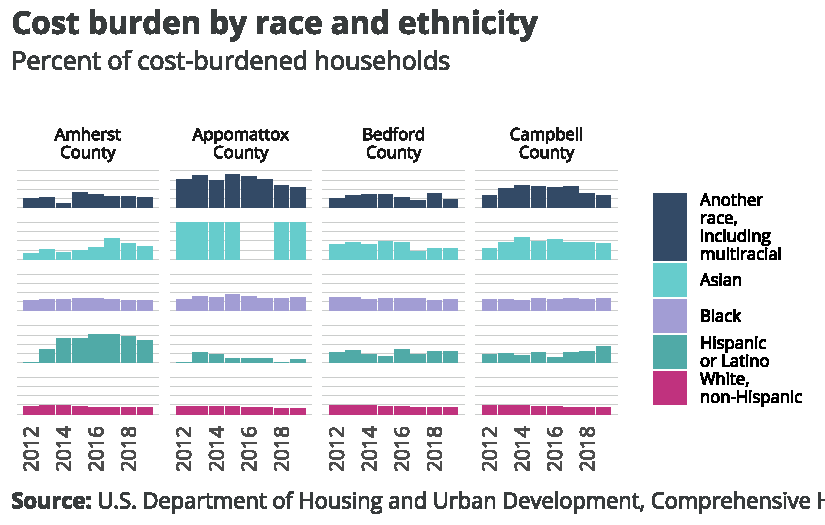
\includegraphics{./part-3-2_files/figure-pdf/fig-cb-race-1.pdf}

}

\caption{\label{fig-cb-race}Local cost burden by race and ethnicity}

\end{figure}

\begin{figure}[H]

{\centering \includegraphics{./part-3-2_files/figure-pdf/fig-gap-1.pdf}

}

\caption{\label{fig-gap}Local rental housing gap by AMI}

\end{figure}

\hypertarget{city-of-lynchburg-housing-market-analysis}{%
\chapter{City of Lynchburg Housing Market
Analysis}\label{city-of-lynchburg-housing-market-analysis}}

The following provides an analysis of major trends impacting housing
within the City of Lynchburg.

\hypertarget{takeaways-2}{%
\section{Takeaways}\label{takeaways-2}}

\hypertarget{population-trends-2}{%
\section{Population trends}\label{population-trends-2}}

\begin{figure}[H]

{\centering \includegraphics{./part-3-3_files/figure-pdf/fig-pop-2020-1.pdf}

}

\caption{\label{fig-pop-2020}Lynchburg estimated and projected
population}

\end{figure}

\begin{figure}[H]

{\centering \includegraphics{./part-3-3_files/figure-pdf/fig-local-chg-1.pdf}

}

\caption{\label{fig-local-chg}Components of population change in
Lynchburg}

\end{figure}

\hypertarget{household-trends-2}{%
\section{Household trends}\label{household-trends-2}}

\begin{figure}[H]

{\centering \includegraphics{./part-3-3_files/figure-pdf/fig-tenure-1.pdf}

}

\caption{\label{fig-tenure}Change in households by tenure in Lynchburg}

\end{figure}

\begin{figure}[H]

{\centering \includegraphics{./part-3-3_files/figure-pdf/fig-age-1.pdf}

}

\caption{\label{fig-age}Households by tenure and age in Lynchburg}

\end{figure}

\begin{figure}[H]

{\centering \includegraphics{./part-3-3_files/figure-pdf/figsize-1.pdf}

}

\caption{Change in households by size and tenure in Lynchburg}

\end{figure}

\begin{figure}[H]

{\centering \includegraphics{./part-3-3_files/figure-pdf/fig-senior-1.pdf}

}

\caption{\label{fig-senior}Change in senior population in Lynchburg}

\end{figure}

\begin{figure}[H]

{\centering \includegraphics{./part-3-3_files/figure-pdf/fig-subfam-1.pdf}

}

\caption{\label{fig-subfam}Change in families living with others in
Lynchburg}

\end{figure}

\begin{figure}[H]

{\centering \includegraphics{./part-3-3_files/figure-pdf/fig-achild-1.pdf}

}

\caption{\label{fig-achild}Cumulative change in adult children living
with parents in Lynchburg}

\end{figure}

\hypertarget{economic-trends-2}{%
\section{Economic trends}\label{economic-trends-2}}

\begin{figure}[H]

{\centering \includegraphics{./part-3-3_files/figure-pdf/fig-inc-dist-1.pdf}

}

\caption{\label{fig-inc-dist}Income distribution by tenure in Lynchburg}

\end{figure}

\begin{figure}[H]

{\centering \includegraphics{./part-3-3_files/figure-pdf/fig-med-inc-1.pdf}

}

\caption{\label{fig-med-inc}Median household income by tenure in
Lynchburg}

\end{figure}

\begin{figure}[H]

{\centering \includegraphics{./part-3-3_files/figure-pdf/fig-race-inc-1.pdf}

}

\caption{\label{fig-race-inc}Median household income by race and
ethnicity in Lynchburg}

\end{figure}

\hypertarget{housing-stock-2}{%
\section{Housing stock}\label{housing-stock-2}}

\begin{figure}[H]

{\centering \includegraphics{./part-3-3_files/figure-pdf/fig-structure-1.pdf}

}

\caption{\label{fig-structure}Distribution of housing stock in Lynchburg
in relation to the region}

\end{figure}

\begin{figure}[H]

{\centering \includegraphics{./part-3-3_files/figure-pdf/fig-mhc-1.pdf}

}

\caption{\label{fig-mhc}Map of manufactured home communities in
Lynchburg}

\end{figure}

\begin{figure}[H]

{\centering \includegraphics{./part-3-3_files/figure-pdf/fig-mhc-county-1.pdf}

}

\caption{\label{fig-mhc-county}Manufactured home communities by size in
Lynchburg}

\end{figure}

\begin{figure}[H]

{\centering \includegraphics{./part-3-3_files/figure-pdf/fig-bps-1.pdf}

}

\caption{\label{fig-bps}Residential building permits by unit type in
Lynchburg}

\end{figure}

\hypertarget{homeownership-market-2}{%
\section{Homeownership market}\label{homeownership-market-2}}

\begin{figure}[H]

{\centering \includegraphics{./part-3-3_files/figure-pdf/fig-ho-1.pdf}

}

\caption{\label{fig-ho}Homeownership rate in Lynchburg}

\end{figure}

\begin{figure}[H]

{\centering \includegraphics{./part-3-3_files/figure-pdf/fig-lburg-sales-1.pdf}

}

\caption{\label{fig-lburg-sales}Lynchburg median home sales price}

\end{figure}

\begin{figure}[H]

{\centering \includegraphics{./part-3-3_files/figure-pdf/fig-lburg-sold-1.pdf}

}

\caption{\label{fig-lburg-sold}Lynchburg closed home sales}

\end{figure}

\begin{figure}[H]

{\centering \includegraphics{./part-3-3_files/figure-pdf/fig-dom-1.pdf}

}

\caption{\label{fig-dom}Lynchburg average days on market}

\end{figure}

\begin{figure}[H]

{\centering \includegraphics{./part-3-3_files/figure-pdf/fig-lburg_sales-1.pdf}

}

\caption{\label{fig-lburg_sales}Map of home sales in Lynchburg}

\end{figure}

\hypertarget{rental-market-2}{%
\section{Rental market}\label{rental-market-2}}

\begin{figure}[H]

{\centering \includegraphics{./part-3-3_files/figure-pdf/fig-rent-1.pdf}

}

\caption{\label{fig-rent}Quarterly average market asking rent in
Lynchburg}

\end{figure}

\begin{figure}[H]

{\centering \includegraphics{./part-3-3_files/figure-pdf/fig-sfr-1.pdf}

}

\caption{\label{fig-sfr}Map of single-family detached rentals in
Lynchburg}

\end{figure}

\begin{figure}[H]

{\centering \includegraphics{./part-3-3_files/figure-pdf/fig-sfr-ward-1.pdf}

}

\caption{\label{fig-sfr-ward}Single-family detached rentals by Lynchburg
ward}

\end{figure}

\begin{figure}[H]

{\centering \includegraphics{./part-3-3_files/figure-pdf/fig-lihtc-exp-1.pdf}

}

\caption{\label{fig-lihtc-exp}LIHTC units by affordability commitment
expiration in Lynchburg}

\end{figure}

\begin{figure}[H]

{\centering \includegraphics{./part-3-3_files/figure-pdf/fig-gap-1.pdf}

}

\caption{\label{fig-gap}Rental housing gap by AMI in Lynchburg}

\end{figure}

\begin{figure}[H]

{\centering \includegraphics{./part-3-3_files/figure-pdf/fig-hcv-map-1.pdf}

}

\caption{\label{fig-hcv-map}Housing Choice Voucher utilization in
Lynchburg}

\end{figure}

\begin{figure}[H]

{\centering \includegraphics{./part-3-3_files/figure-pdf/fig-cb-tenure-1.pdf}

}

\caption{\label{fig-cb-tenure}Lynchburg cost burden by tenure}

\end{figure}

\begin{figure}[H]

{\centering \includegraphics{./part-3-3_files/figure-pdf/fig-cb-race-1.pdf}

}

\caption{\label{fig-cb-race}Lynchburg cost burden by race and ethnicity}

\end{figure}

\part{Part 4: Policy evaluation}

\hypertarget{policy-evaluation}{%
\chapter{Policy Evaluation}\label{policy-evaluation}}

\part{Part 5: Policy recommendations}

\hypertarget{regional-solutions}{%
\chapter{Regional Solutions}\label{regional-solutions}}

\hypertarget{local-solutions}{%
\chapter{Local Solutions}\label{local-solutions}}

\part{Appendix}



\end{document}
